%%%%%%%%%%%%%%%%%%%%%%%%%%%%%%%%%%%%%%%%%
% Article EcoFoG
% Version 2.1 (23/10/2017)
%
% adapté de :
% Stylish Article
% LaTeX Template
% Version 1.0 (31/1/13)
%
% This template has been downloaded from:
% http://www.LaTeXTemplates.com
%
% Original author:
% Mathias Legrand (legrand.mathias@gmail.com)
%
% License:
% CC BY-NC-SA 3.0 (http://creativecommons.org/licenses/by-nc-sa/3.0/)
%
%%%%%%%%%%%%%%%%%%%%%%%%%%%%%%%%%%%%%%%%%


%----------------------------------------------------------------------------------------
%	PACKAGES AND OTHER DOCUMENT CONFIGURATIONS
%----------------------------------------------------------------------------------------

\documentclass[fleqn,10pt]{ArtEcoFoG} % Document font size and equations flushed left

\setcounter{tocdepth}{3} % Show only three levels in the table of contents section: sections, subsections and subsubsections


% Pandoc environments
\usepackage{framed}
\usepackage{fancyvrb}
\providecommand{\tightlist}{%
  \setlength{\itemsep}{0pt}\setlength{\parskip}{0pt}}
\newcommand{\VerbBar}{|}
\newcommand{\VERB}{\Verb[commandchars=\\\{\}]}
\DefineVerbatimEnvironment{Highlighting}{Verbatim}{commandchars=\\\{\}, fontsize=\scriptsize} % Code R
\definecolor{shadecolor}{RGB}{248,248,248}
\newenvironment{Shaded}{\begin{snugshade}}{\end{snugshade}}
\newcommand{\KeywordTok}[1]{\textcolor[rgb]{0.13,0.29,0.53}{\textbf{{#1}}}}
\newcommand{\DataTypeTok}[1]{\textcolor[rgb]{0.13,0.29,0.53}{{#1}}}
\newcommand{\DecValTok}[1]{\textcolor[rgb]{0.00,0.00,0.81}{{#1}}}
\newcommand{\BaseNTok}[1]{\textcolor[rgb]{0.00,0.00,0.81}{{#1}}}
\newcommand{\FloatTok}[1]{\textcolor[rgb]{0.00,0.00,0.81}{{#1}}}
\newcommand{\ConstantTok}[1]{\textcolor[rgb]{0.00,0.00,0.00}{{#1}}}
\newcommand{\CharTok}[1]{\textcolor[rgb]{0.31,0.60,0.02}{{#1}}}
\newcommand{\SpecialCharTok}[1]{\textcolor[rgb]{0.00,0.00,0.00}{{#1}}}
\newcommand{\StringTok}[1]{\textcolor[rgb]{0.31,0.60,0.02}{{#1}}}
\newcommand{\VerbatimStringTok}[1]{\textcolor[rgb]{0.31,0.60,0.02}{{#1}}}
\newcommand{\SpecialStringTok}[1]{\textcolor[rgb]{0.31,0.60,0.02}{{#1}}}
\newcommand{\ImportTok}[1]{{#1}}
\newcommand{\CommentTok}[1]{\textcolor[rgb]{0.56,0.35,0.01}{\textit{{#1}}}}
\newcommand{\DocumentationTok}[1]{\textcolor[rgb]{0.56,0.35,0.01}{\textbf{\textit{{#1}}}}}
\newcommand{\AnnotationTok}[1]{\textcolor[rgb]{0.56,0.35,0.01}{\textbf{\textit{{#1}}}}}
\newcommand{\CommentVarTok}[1]{\textcolor[rgb]{0.56,0.35,0.01}{\textbf{\textit{{#1}}}}}
\newcommand{\OtherTok}[1]{\textcolor[rgb]{0.56,0.35,0.01}{{#1}}}
\newcommand{\FunctionTok}[1]{\textcolor[rgb]{0.00,0.00,0.00}{{#1}}}
\newcommand{\VariableTok}[1]{\textcolor[rgb]{0.00,0.00,0.00}{{#1}}}
\newcommand{\ControlFlowTok}[1]{\textcolor[rgb]{0.13,0.29,0.53}{\textbf{{#1}}}}
\newcommand{\OperatorTok}[1]{\textcolor[rgb]{0.81,0.36,0.00}{\textbf{{#1}}}}
\newcommand{\BuiltInTok}[1]{{#1}}
\newcommand{\ExtensionTok}[1]{{#1}}
\newcommand{\PreprocessorTok}[1]{\textcolor[rgb]{0.56,0.35,0.01}{\textit{{#1}}}}
\newcommand{\AttributeTok}[1]{\textcolor[rgb]{0.77,0.63,0.00}{{#1}}}
\newcommand{\RegionMarkerTok}[1]{{#1}}
\newcommand{\InformationTok}[1]{\textcolor[rgb]{0.56,0.35,0.01}{\textbf{\textit{{#1}}}}}
\newcommand{\WarningTok}[1]{\textcolor[rgb]{0.56,0.35,0.01}{\textbf{\textit{{#1}}}}}
\newcommand{\AlertTok}[1]{\textcolor[rgb]{0.94,0.16,0.16}{{#1}}}
\newcommand{\ErrorTok}[1]{\textcolor[rgb]{0.64,0.00,0.00}{\textbf{{#1}}}}
\newcommand{\NormalTok}[1]{{#1}}
\usepackage{longtable,booktabs}
\usepackage{caption}
% These lines are needed to make table captions work with longtable:
\makeatletter
\def\fnum@table{\tablename~\thetable}
\makeatother
% longtable 2 columns
% https://tex.stackexchange.com/questions/161431/how-to-solve-longtable-is-not-in-1-column-mode-error
\makeatletter
\let\oldlt\longtable
\let\endoldlt\endlongtable
\def\longtable{\@ifnextchar[\longtable@i \longtable@ii}
\def\longtable@i[#1]{\begin{figure}[t]
\onecolumn
\begin{minipage}{0.5\textwidth}\scriptsize
\oldlt[#1]
}
\def\longtable@ii{\begin{figure}[t]
\onecolumn
\begin{minipage}{0.5\textwidth}\scriptsize
\oldlt
}
\def\endlongtable{\endoldlt
\end{minipage}
\twocolumn
\end{figure}}
\makeatother

\usepackage{graphicx,grffile}
\makeatletter
\def\maxwidth{\ifdim\Gin@nat@width>\linewidth\linewidth\else\Gin@nat@width\fi}
\def\maxheight{\ifdim\Gin@nat@height>\textheight0.8\textheight\else\Gin@nat@height\fi}
\makeatother
% Scale images if necessary, so that they will not overflow the page
% margins by default, and it is still possible to overwrite the defaults
% using explicit options in \includegraphics[width, height, ...]{}
\setkeys{Gin}{width=\maxwidth,height=\maxheight,keepaspectratio}

% User-adder preamble
\usepackage{textcomp} \DeclareUnicodeCharacter{B0}{\textdegree}
\usepackage{tabu} \usepackage{caption}
\captionsetup{justification = justified}
\renewenvironment{table}{\begin{table*}}{\end{table*}\ignorespacesafterend}
\hyphenation{bio-di-ver-si-ty sap-lings re-or-gan-i-za-tion post-dis-tur-bance dis-tur-bance}

%----------------------------------------------------------------------------------------
%	ARTICLE INFORMATION
%----------------------------------------------------------------------------------------

\JournalInfo{\ }
\Archive{\ }

\PaperTitle{Post-Disturbance Tree Community Trajectories in a Neotropical Forest} % Article title

\Authors{
Ariane MIRABEL\textsuperscript{1*}\\ Bruno Herault\textsuperscript{2}\\ Eric Marcon\textsuperscript{1}
} % Authors
\affiliation{
\textsuperscript{1}UMR EcoFoG, AgroParistech, CNRS, Cirad, INRA, Université des Antilles,
Université de Guyane.\\ \hspace{1em} Campus Agronomique, 97310 Kourou, France.\\\textsuperscript{2}INPHB, Institut National Polytechnique Félix Houphoüet-Boigny\\ \hspace{1em} Yamoussoukro, Ivory Coast.
}
\affiliation{*\textbf{Corresponding author}: ariane.mirabel@ecofog.gf, https://github.com/ArianeMirabel} % Corresponding author

\Keywords{Community Ecology, Disturbance Trajectories, Intermediate Disturbance Hypothesis, Mid-term Resilience, Neotropical Forests, Taxonomic and Functional Biodiversity} % Keywords - if you don't want any simply remove all the text between the curly brackets
\newcommand{\keywordname}{Keywords} % Defines the keywords heading name

%----------------------------------------------------------------------------------------
%	ABSTRACT
%----------------------------------------------------------------------------------------

\Abstract{
Understand biodiversity trajectories of tropical forests following
disturbance and clarify the link between biodiversity and disturbance is
urgent to anticipate the impact of the global change context. This calls
to highlight the taxonomic and functional facets of tree community
trajectories and the underlying processes, and to clarify the link
between biodiversity and disturbance, specifically the scope of the
Intermediate Disturbance Hypothesis (IDH) that is debated tropical
forests. In this study, we analyzed tree community response to a
disturbance gradient in a Neotropical forest through diversity,
composition and redundancy post-disturbance trajectories over 30 years.
We considered taxonomic trajectories and functional trajectories based
on 7 leaf, stem and life-history traits. While taxonomic trajectories
differed among communities, functional trajectories remained similar and
convergent, and this decoupling was explained by the variations in
community functional redundancy mitigating the functional impact of
disturbance. We validated the IDH, based on an intensity threshold of
20-25\% of AGB removed, and we clarified its scope, showing that it
applied to taxonomic but not functional diversity, and applied around 20
years after disturbance when the recruitment of pioneers and
late-successionals were balanced. Although consistent, the recovery of
community composition, diversity and redundancy remained unachieved
after 30 years. This acknowledged the need of decades-long cycles
without disturbance to ensure a complete recovery, and questioned
tropical forest community resilience after repeated disturbances.
}

%----------------------------------------------------------------------------------------

\begin{document}

\selectlanguage{english}

\flushbottom % Makes all text pages the same height

\maketitle % Print the title and abstract box

\tableofcontents % Print the contents section

\thispagestyle{empty} % Removes page numbering from the first page

%----------------------------------------------------------------------------------------
%	ARTICLE CONTENTS
%----------------------------------------------------------------------------------------
























\section{Introduction}\label{introduction}

The large areas covered with tropical forests worldwide hold crucial
environmental, economic and social values. They provide wood and
multiple non-timber forest products, shelter a diversified fauna, and
ensure cultural and human well-being. They regulate as well the local
and regional climates, and the carbon, water and nutrient cycles.
However, the growing demand in forests products together with current
global changes increase the pressure on remaining natural forests
\citep{Morales-Hidalgo2015}. These threats affect the natural
disturbance regime that shape and maintain the structure, composition
and functioning of tree communities
\citep{Schnitzer2001, Anderson-Teixeira2013, Sist2015}. It is urgent to
understand community response to disturbance and the underlying
processes to anticipate the fate of tropical forests in the current
context. Disturbance change both community abiotic and biotic
environments, through modifications in the fluxes of light, heat and
water \citep{Goulamoussene2017}. In tropical forests, the forest
environment is maintained after disturbance and there is a suit of
changes in the structure and functioning of communities that consitutes
a secondary succession. For now, this succession has been largely
studied through post-disturbance trajectories of forest structural
parameters such as aboveground biomass, tree height or stem density
\citep{Piponiot2016, Rutishauser2016}. Models based on observed
trajectories then assessed community time to recovery and identified
some of the determinants of post-disturbance trajectories, like forest
structure, forest composition, environmental parameters and disturbance
characteristics \citep{Herault2018}. Regarding community diversity and
composition, however, post-disturbance trajectories have not been as
thoroughly understood \citep{Guitet2018, Molino2001}. Given the variety
of species response to disturbance and the huge diversity of tropical
forests, post-disturbance biodiversity trajectories might be very
diverse \citep{Lindenmayer2012, Garcia_florez2017}. It is essential to
anticipate these trajectories and highlight the link between
biodiversity and disturbance, and specifically how disturbance intensity
and frequency determine the rate, endpoint and duration of
post-disturbance trajectories \citep{Chazdon2003a, Willig2018}.

An early conceptual basis of the linkage between biodiversity and
disturbance is the Intermediate Disturbance Hypothesis (IDH). The IDH
assumes a relationship between community diversity and the intensity and
frequency of disturbance events \citep{Connell1978}. The theory and
states that community diversity peaks at intermediate level of
disturbance. The fluctuations of environmental conditions after
disturbance are assumed to prevent competitive exclusion in fostering
both competitively superior species and fast colonizers
\citep{Shea2004, Pulsford2016}. In tropical forests, however,
observations of the IDH are often blurry compared to theoretical
expectations \citep{Hugues2007, Sheil2003, Norden2017}, and the
validation of the theory remains controversial
\citep{Hubbell2001, Fox2013, Sheil2013}. The link between biodiversity
and disturbance might be complicated by the huge diversity of tropical
communities and a variety of ecological processes may underlie the IDH
(colonisation, facilitation,
coexistence,etc)\citep{Lindenmayer2012, Garcia_florez2017}. There is a
need to clarify the scope of the IDH in terms of the different facets of
community diversity, that are the taxonomic richness, the species
abundance distribution and the community functioning. Besides, there is
a need to delineate the scope of the IDH in time, and highlight the
moment when the conditions for the IDH emerge
\citep{Sheil2003, Shea2004}.

Analysing community response to disturbance requires a set of metrics,
to grasp all aspects of community changes
\citep{Sheil2003, Shea2004, Mayfield2010}. The analysis should first
consider community composition, which is crucial for conservation issues
and reveals the species fostered by the disturbance
\citep{Lavorel2002, Bellwood2006}. Then, diversity metrics encompassing
taxonomic richness and evenness should be considered to assess the
changes in community abundance distribution. A functional approach, that
account for species biological attributes and ecological strategy, would
directly link community diversity, composition and redundancy to
ecosystem functioning and environmental constraints
\citep{Violle2007b, Baraloto2012a}. In that respect, a vast literature
allowed recognizing major traits that represent species ecological
strategy and determine how they respond to changing conditions
\citep{Diaz2005}. Specifically in tropical forests, the functional
approach revealed the post-disturbance deterministic processes entailing
a shift from a dominance of ``conservative'' slow-growing species
dealing with scarce resources, to a dominance of ``acquisitive''
fast-growing species with rapid and efficient use of abundant resources
\citep{Rees2001, Reich2014, Herault2011}. This shift is translated into
the trajectories of average community value of key functional traits
related to resource acquisition (leaf and stem traits) and life-history
strategy (seed mass, maximum size)
\citep{Wright2004, TerSteege2006, Westoby2006a, Chave2009b}. The
functional approach also encompasses the analysis of functional
redundancy, that quantifies the amount of shared trait values among
species \citep{Carmona2016}. The typical high functional redundancy of
hyper-diverse tropical forests \citep{Bellwood2006} mitigates the
impacts of species removal on ecosystem functioning and determines
communities resilience after disturbance \citep{Elmqvist2003, Diaz2005}.

In this study, we monitored over 30 years the response of 75 ha of
Neotropical forest plots set up on a gradient of disturbance intensity,
from 10 to 60\% of above-ground biomass (AGB) loss. We made use of a
large functional traits database encompassing major leaf, stem and
life-history traits in order to draw the taxonomic and functional
trajectories in terms of richness, evenness, composition and redundancy.
Specifically, (i) we defined taxonomic and functional post-disturbance
trajectories and examined the underlying ecological process, (ii) we
discussed the scope of the IDH regarding the different facets of
community diversity and the time after disturbance, and (iii) we
analyzed community resilience and time to recovery.

\section{Material and Methods}\label{material-and-methods}

\subsection{Study site}\label{study-site}

Paracou station in French Guiana (5\textdegree 18'N and
52\textdegree 53'W) is located in a lowland tropical rain forest in a
tropical wet climate with mean annual temperature of 26\textdegree C,
mean annual precipitation averaging 2980 mm.y\textsuperscript{-1} (30-y
period) and a 3-month dry season (\textless{} 100
mm.month\textsuperscript{-1}) from mid-August to mid-November, and a
one-month dry season in March \citep{Wagner2011}. Elevation ranges from
5 to 50 m and mean annual temperature is 26°C. Soils are thin ferralitic
acrisols over a layer of transformed saprolite. The ferralitic surface
is thin in the whole area, with low permeability and lateral drainage,
except in the highest hilltops where it is thick and with a free
vertical drainage \citep{Gourlet-Fleury2004}.

The experiment is a network of 12 6.25 ha plots that underwent a
disturbance gradient of three logging, thinning and fuelwood cutting
treatments (Table \ref{tab:Tab1}) according to a randomized plot design
with three replicate blocks of four plots. The disturbance corresponds
to an intensity gradient. For treatment 1 (T1) 10 trees of commercial
species (of a diameter at 1.3 m height (DBH) equal or above 50 cm) were
felled per hectare. For treatment 2 (T2) 10 trees/ha of commercial
species (DBH \(\geq\) 50 cm) were felled and 30 trees/ha of non-valuable
species (DBH \(\geq\) 40 cm) were removed by poison girdling. For
treatment 3 (T3) 10 trees/ha of commercial species (DBH \(\geq\) 50 cm)
were felled and 30 trees/ha of non-valuable species (15 with DBH
\(\geq\) 50 cm and 15 with DBH \(\geq\) 40 cm) were removed by poison
girdling \citep{Schmitt1990}. Disturbance intensity was measured as the
percentage of aboveground biomass (\%AGB) lost between the first
inventory in 1984 and five years after disturbance \citep{Piponiot2016}
estimated with the BIOMASS R package \citep{Biomass2018}.

\begin{table}

\caption{\label{tab:Tab1}Intervention table, summary of the disturbance intensity for the 4 plot treatments in Paracou.}
\centering
\begin{tabu} to \linewidth {>{\raggedright}X>{\raggedright}X>{\raggedright}X>{\raggedright}X>{\raggedright}X}
\toprule
Treatment & Timber & Thinning & Fuelwood & \%AGB lost\\
\midrule
Control & - & - & - & 0\\
T1, low & DBH $\geq$ 50 cm, commercial species, $\approx$ 10   $trees.ha^{-1}$ & - & - & $[12-33]$\\
T2, intermediate & DBH $\geq$ 50 cm, commercial species, $\approx$ 10  $trees.ha^{-1}$ & DBH $\geq$ 40 cm, non-valuable species, $\approx$ 30   $trees.ha^{-1}$ & - & $[33-56]$\\
T3, high & DBH $\geq$ 50 cm, commercial species, $\approx$ 10  $trees.ha^{-1}$ & DBH $\geq$ 50 cm, non-valuable species, $\approx$ 15  $trees.ha^{-1}$ & 40 cm $\leq$ DBH $\leq$ 50 cm, non-valuable species,\ $\approx$ 15 $trees.ha^{-1}$ & $[35-56]$\\
\bottomrule
\end{tabu}
\end{table}

\subsection{Inventories protocol and dataset
collection}\label{inventories-protocol-and-dataset-collection}

The study site corresponds to a tropical rainforest typical of the
Guiana Shield with a dominance of \emph{Fabaceae},
\emph{Chrysobalanaceae}, \emph{Lecythidaceae} and \emph{Sapotaceae}. In
the 12 experimental plots, all trees above 10 cm DBH have been mapped
and measured annually since 1984. Trees are first identified with a
vernacular name assigned by the forest worker team, and afterward with a
scientific name assigned by botanists during regular botanical
campaigns. In 1984, specific vernacular names were given to 62
commercial or common species whereas more infrequent ones were
identified under general identifiers only distinguishing trees and
palms. From 2003, botanical campaigns have been conducted every 5 to 6
years to identify all trees at the species level but identification
levels still varied among plots and campaigns.

This variability of protocols in time raised methodological issues as
vernacular names usually correspond to different botanical species. This
resulted in significant taxonomic uncertainty that had to be propagated
to composition and diversity metrics. The uncertainty propagation was
done through a Bayesian framework reconstituting complete inventories at
genus level from real incomplete ones on the basis of
vernacular/botanical names association. Vernacular names were replaced
through multinomial trials based on the association probability
\(\big[\alpha_1, \alpha_2,..., \alpha_V\big]\) observed across all
inventories between each vernacular name \emph{v} and all species
\(\big[s_1, s_2,..., s_N\big]\):

\begin{align}
M_v\Big(\big[s_1, s_2,..., s_N\big],\big[\alpha_1, \alpha_2,..., \alpha_V\big]\Big) \nonumber
\end{align}

See Supplementary Materials -Fig. S1 and \citet{Aubry-Kientz2013} for
the detailed methodology.

Six functional traits representing leaf economics (leaf thickness,
toughness, total chlorophyll content and specific leaf area) and stem
economics (wood specific gravity and bark thickness), and life-history
traits (maximum specific height and seed mass) came from the BRIDGE
project \footnote{http://www.ecofog.gf/Bridge/}. Trait values were
assessed from a selection of individuals located in nine permanent plots
in French Guiana, including two in Paracou, and comprised 294 species
pertaining to 157 genera. Missing trait values (10\%) were filled using
multivariate imputation by chained equation \citep{Mice2011}.
Imputations were restricted within genus or family when samples were too
scarce, in order to account for the phylogenetic signal. Whenever a
species was not in the dataset, it was attributed a set of trait values
randomly sampled among species of the next higher taxonomic level (same
genus or family). As seed mass information was classified into classes,
no data filling process was applied and analyses were restricted to the
414 botanical species recorded.

All composition and diversity metrics were obtained after 50 iterations
of the uncertainty propagation framework.

\subsection{Composition and diversity
metrics}\label{composition-and-diversity-metrics}

Because of the variability in the precision of botanical identification
efforts, we were constraint to conduct the taxonomic composition and
diversity analysis at the genus level. Taxonomic and functional
trajectories of community composition were followed in a two-dimensional
NMDS ordination plan. Two NMDS using abundance-based (Bray-Curtis)
dissimilarity measures were conducted to map either taxonomic or
functional composition, the latter based on the seven leaf, stem and
life history traits (without seed mass classes). Trajectories along time
were reported through the Euclidean distance between the target
inventories and the reference inventories in 1989, \emph{i.e.} 2 years
after disturbance. Univariate trajectories of the leaf, stem and
life-history traits were also visualized with the community weighted
means (CWM) \citep{Diaz2007}. Species seed mass were given in 5 mass
classes. Seed mass trajectories were therefore reported as the
proportion of each class in the inventories (Supplementary materials).

The taxonomic diversity was reported through species richness and the
Hill number translation of the Simpson index \citep{Hill1973}. These
metrics allowed assessing the taxonomic richness as well as evenness,
through the comparison between richness and Simpson diversity. R.esults
will thus be discussed directly in terms of taxonomic richness and
evenness. Both indices belong to the set of HCDT or generalized entropy,
respectively corresponding to the 0 and 2 order of diversity (q),
recommended for diversity studies \citep{Marcon2015b}. The functional
diversity was reported using the functional richness and functional
evenness, \emph{i.e} the Rao index of quadratic entropy. The Rao index
combines species abundance distribution, and the average pairwise
functional dissimilarity between species computed by the gower distance.

The impacts of initial disturbance were tested with the Spearman rank
correlation between the extremes of taxonomic and functional metrics
reached over the 30 years and the initial \%AGB loss. They were besides
analyzed through polynomial regression between (i) taxonomic and
functional richness and evenness and (ii) the initial \%AGB loss at 10,
20 and 30 years after disturbance.

Functional redundancy was measured as the overlap among species in
community functional space \citep{Carmona2016}. First, the individuals
of the trait database were mapped in the plane of the two first axes
from a PCA analysis. Then, for each species, the traits probability
density (TPD) were computed through two-dimension kernel density
estimators. Second, for each community, the TDB weigthed by species
abundance were summed accross the functional space. Third, the
functional space was divided into a 100 x 100 grid and the number of
species with a positive TDP was counted in each cell. The average count
across cells minus 1 returnedthe Community Functional Redundancy, which
was the average number of species in the community that share the same
trait values.

\section{Results}\label{results}

\subsection{Community Composition}\label{community-composition}

From 1989 (2 years after disturbance) to 2015 (28 years after
disturbance), 828 388 individual trees and 591 botanical species
pertaining to 223 genera and 64 families were recorded.

While both taxonomic and functional composition remained stable in
undisturbed communities (Fig. \ref{fig:NMDSplans}), they followed marked
and consistent trajectories over post-\break disturbance time. In
disturbed communities, these compositional changes corresponded to
shifts towards species with more acquisitive functional strategies, from
communities with high mean WSG to high mean SLA and chlorophyll content
(see appendix I). For functional composition, this translated into
cyclic compositional changes with an incomplete recovery of the initial
composition (Fig. \ref{fig:NMDSplans}). The maximum dissimilarity with
the initial state was positively correlated with the disturbance
intensity for both taxonomic and functional composition
(\(\rho_{Spearman}^{Taxonomic}=0.87\) and
\(\rho_{Spearman}^{Functional}=0.90\) respectively). The maximum
dissimilarity with the initial was reached for taxonomic composition
between 15 to 25 years, for most of the plots, and around 22 years for
functional composition.

\begin{figure*}

{\centering 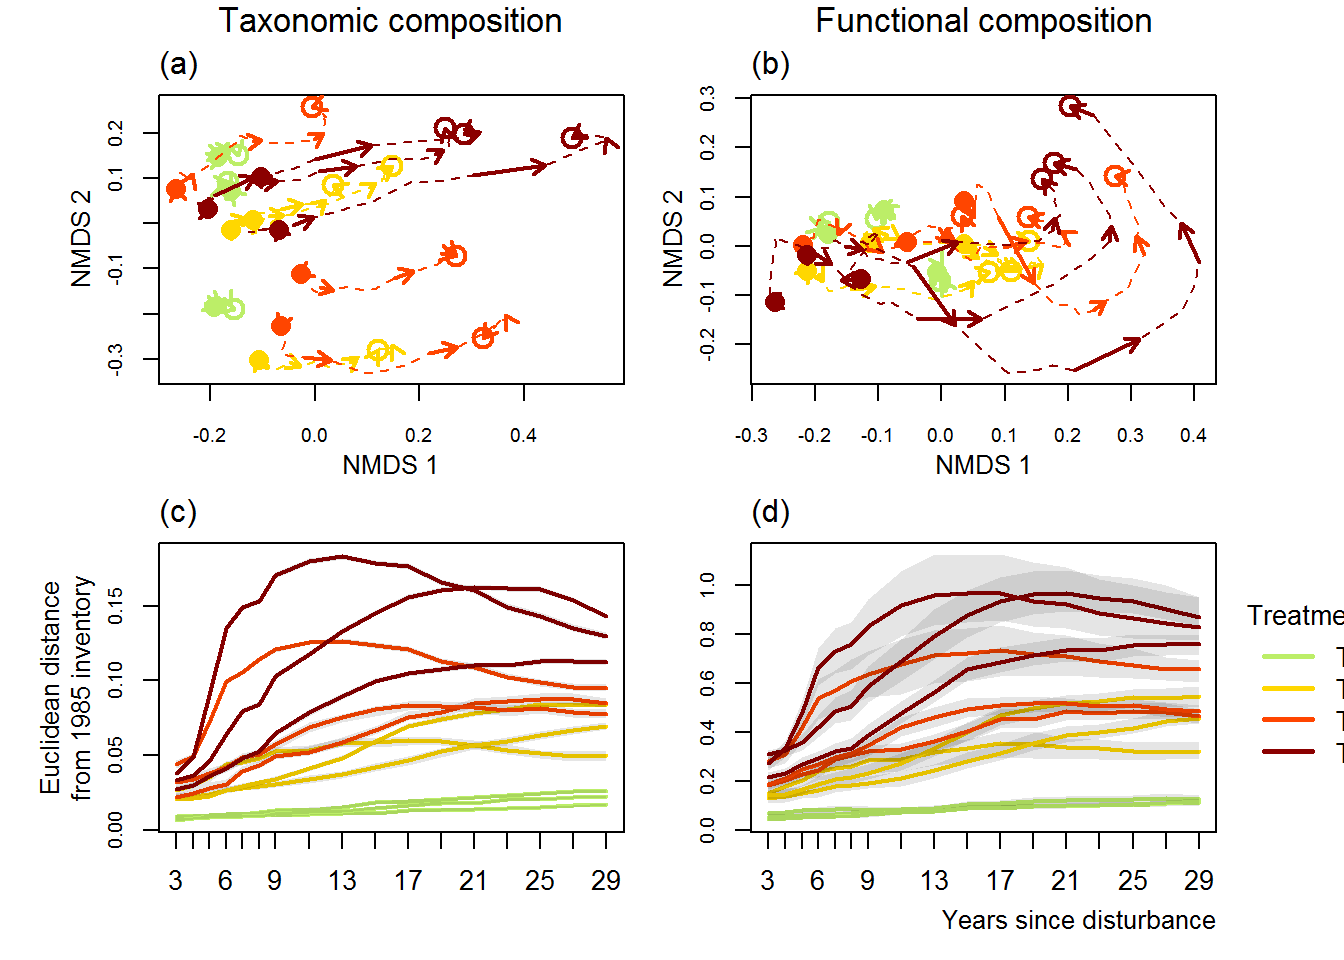
\includegraphics[width=1\linewidth]{WholePlotTrajectories_files/figure-latex/NMDSplans-1} 

}

\caption{Plot trajectories in terms of taxonomic composition (\textbf{(a)} and \textbf{(c)}) and functional composition (\textbf{(b)} and \textbf{(d)}) in a two-dimensional NMDS plan. Lower panels (\textbf{(c)} and \textbf{(d)}) represent the Euclidean distance to initial condition along the 30 sampled years. Shaded areas are the credibility intervals.}\label{fig:NMDSplans}
\end{figure*}

Community CWM average value of all traits and seed mass proportions
followed unimodal trajectories, either stabilizing or returning towards
their initial values, to the exception of leaf chlorophyll content,
which continued to increase for some T3 and T2 plots 30 years after
disturbance.

Community CWM average value of Maximum height at adult stage
(\emph{Hmax}), leaf toughness and wood specific gravity (\emph{WSG})
first decreased and then slightly increased but remained significantly
lower than their initial value (Fig. \ref{fig:CWM}). On the other side,
bark thickness and specific leaf area (\emph{SLA}) increased and while
bark thickness remained substantially high after 30 years, \emph{SLA}
had almost recovered to its initial value. For all traits, the maximum
difference to initial value was correlated to the disturbance intensity.
Positive correlations were observed for Leaf thickness, chlorophyll
content, SLA and bark thickness
(\(\rho_{Spearman}^{Leaf thickness}=0.76\),
\(\rho_{Spearman}^{Chlorophyll content}=0.60\),
\(\rho_{Spearman}^{SLA}=0.93\),
\(\rho_{Spearman}^{Bark thickness}=0.71\)). Negative correlation was
observed for Leaf toughness, WSG and Hmax
(\(\rho_{Spearman}^{Leaf toughness}=-0.53\),
\(\rho_{Spearman}^{WSG}=-0.75\), \(\rho_{Spearman}^{Hmax}=-0.40\)) The
proportions of the three lightest seed mass classes increased in all
disturbed plots, and decreased after 30 years for the lightest class
while it stabilized for the two other (Supp. Mat. - Fig. S2).

\begin{figure*}

{\centering 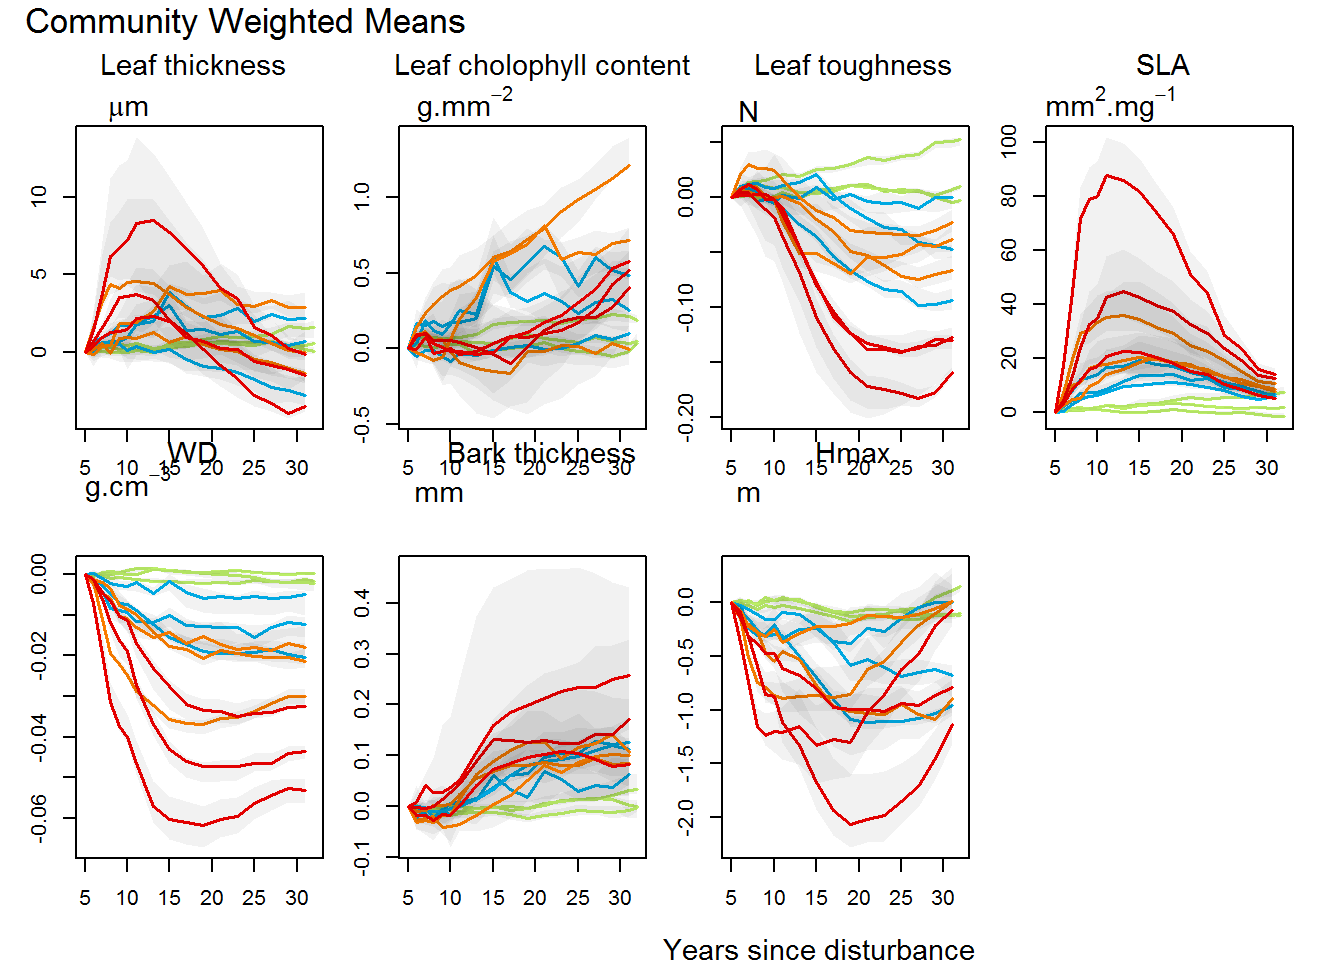
\includegraphics[width=1\linewidth]{WholePlotTrajectories_files/figure-latex/CWM-1} 

}

\caption{Trajectories of community weighted means over 30 years after disturbance of four leaf traits (Leaf thickness, chlorophyll content, toughness, and specific area), two stem traits (wood specific gravity, and bark thickness) and one life history trait (Specific maximum height at adult stage). }\label{fig:CWM}
\end{figure*}

\subsection{Community taxonomic and functional
diversity}\label{community-taxonomic-and-functional-diversity}

For undisturbed plots, taxonomic richness and Simpson diversity remained
stable over the 30 years of monitoring. In disturbed communities, after
low disturbance intensity the taxonomic richness increased, reaching a
maximum gain of 14 botanical genera (plot 3 from treatment 2). After
intense disturbance the taxonomic richness followed a more complex
trajectory, decreasing for ten years after disturbance before recovering
to pre-disturbance values. The maximum richness loss or gain after
disturbance was positively correlated with the disturbance intensity
(\(\rho_{Spearman}^{Richness}=0.50\)). In all disturbed plots the
Simpson diversity first increased until a maximum reached after around
20 years. This maximum was positively correlated with the disturbance
intensity (\(\rho_{Spearman}^{Simpson}=0.77\)). The Simpson diversity
then stabilized except for two T3 plots (plots 8 and 12) for which it
kept increasing (Fig. \ref{fig:DivTaxo}).

\begin{figure*}

{\centering 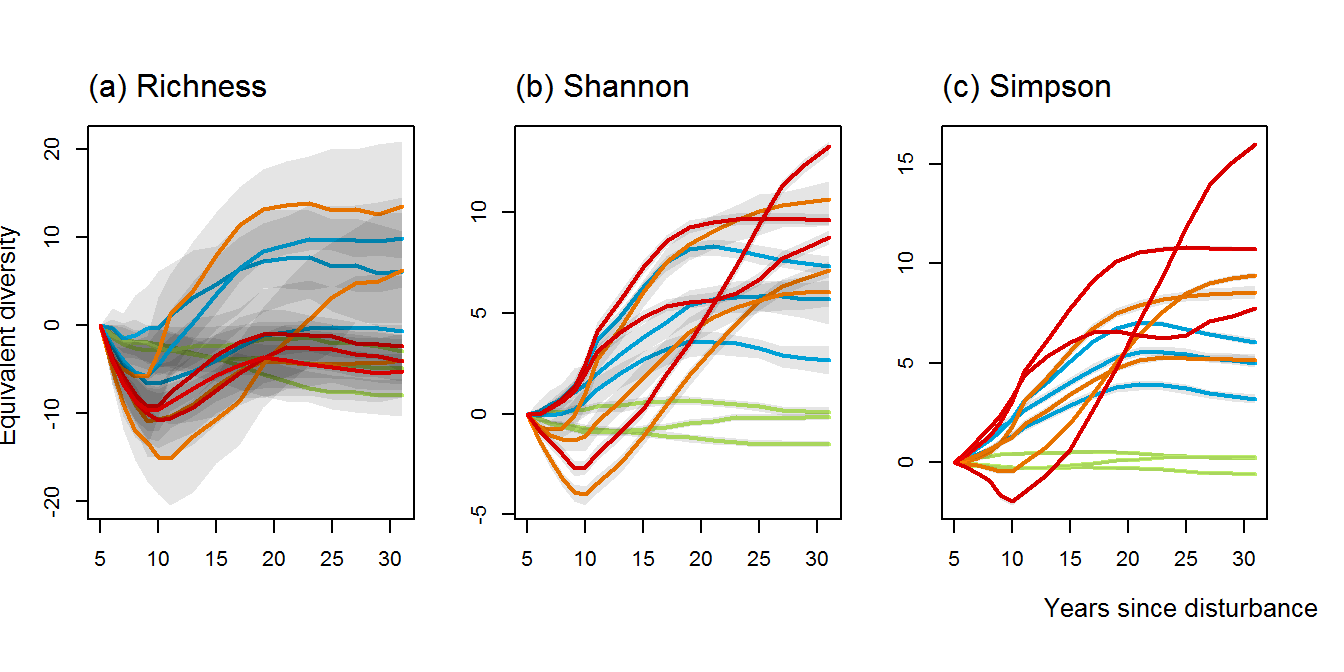
\includegraphics[width=1\linewidth]{WholePlotTrajectories_files/figure-latex/DivTaxo-1} 

}

\caption{Trajectories over 30 years of the difference with the 1989 inventory (2 years after disturbance) of community taxonomic richness \textbf{(a)}, Simpson diversity \textbf{(b)}, functional richness \textbf{(c)}, and Rao diversity \textbf{(d)}. Shaded areas are the credibility intervals }\label{fig:DivTaxo}
\end{figure*}

The plot 7 from treatment 1 displayed constantly outlying functional
richness and Rao diversity and was removed from the graphical
representation for better readability. In undisturbed plots both
functional richness and Rao diversity remained stable along the 30
years. In disturbed plots, both trajectories depended on the disturbance
intensity, with their maximum being positively correlated to \%AGB loss
\(\rho_{Spearman}^{Richness}=0.76\) and \(\rho_{Spearman}^{Rao}=0.60\).
Functional richness and Rao diversity displayed for low disturbance
intensity a low but long-lasting increase up to a maximum reached after
20-25 years, and for high intensity, a fast but short increase followed
after 10 years by a slow decrease towards the initial values.

The second-degree polynomial regressions between (i) the percentage AGB
loss and (ii) taxonomic and functional diversity after 10, 20 and 30
years best predicted the hump-shaped curve of the disturbance impact
along the disturbance intensity gradient \ref{fig:IDHplot}. The
relationship between the disturbance impact and its intensity was more
markedly hump-shaped for the taxonomic richness than for the Simpson
diversity. For both functional richness and Rao diversity the
relationship was almost linear. The regression model better predicted
the functional richness and Rao diversity
(\(0.55<R^2_{Functional Richness}<0.72\), and
\(0.60<R^2_{Functional Rao}<0.81\)) than the taxonomic richness and
evenness (\(0.21<R^2_{Taxonomic Richness}<0.4\), and
\(-0.15<R^2_{Taxonomic Simpson}<0.43\) respectively).

\begin{figure*}

{\centering 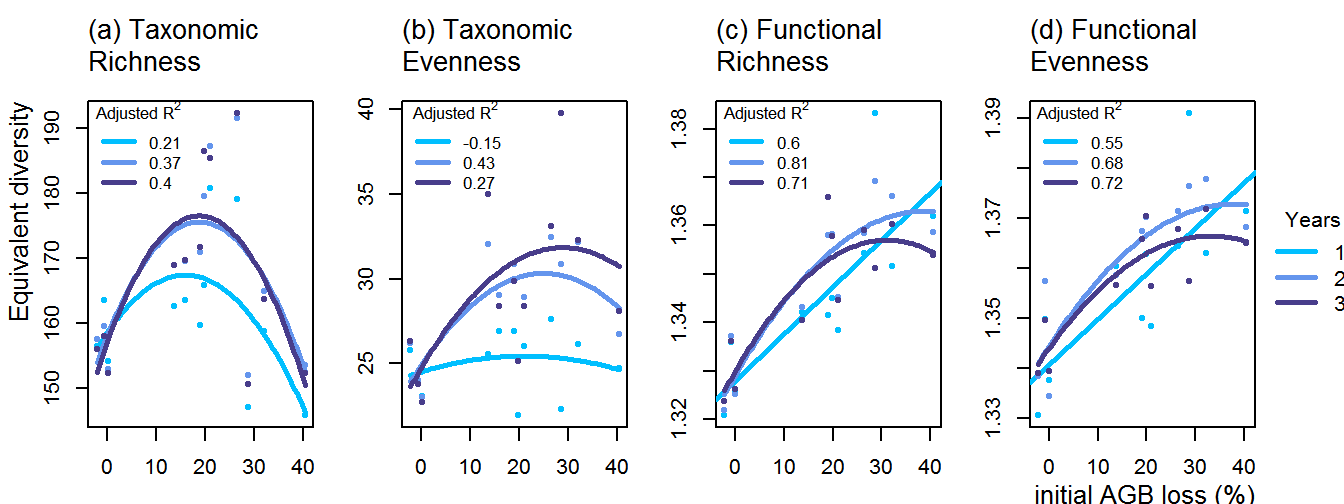
\includegraphics[width=1\linewidth]{WholePlotTrajectories_files/figure-latex/IDHplot-1} 

}

\caption{Relationship between the initial \%AGB loss and community taxonomic richness \textbf{(a)}, taxonomic evenness \textbf{(b)}, functional richness \textbf{(c)},and functional evenness \textbf{(d)} at 10, 20 and 30 years after disturbance}\label{fig:IDHplot}
\end{figure*}

\subsection{Functional redundancy}\label{functional-redundancy}

All disturbed plots had lower functional redundancy than control plots
and followed similar hump-shaped trajectories (\ref{fig:RedFunRest}).
The maximum redundancy loss was positively correlated with the
disturbance intensity (\(\rho_{Spearman}=0.47\)) and the recovery had
not attained initial values for any disturbed communities after 30
years.

\begin{figure}

{\centering 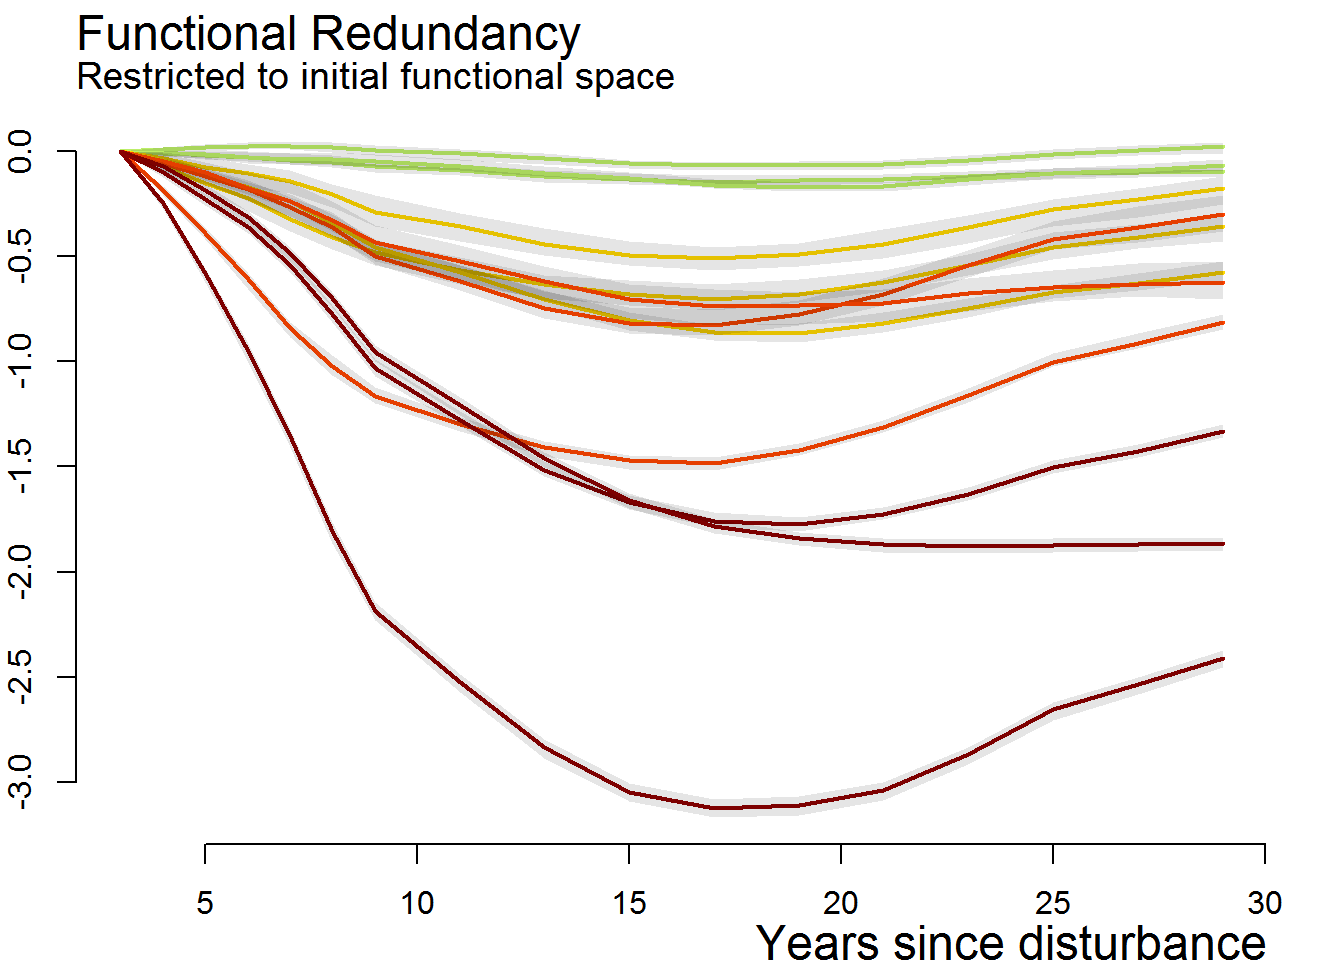
\includegraphics[width=1\linewidth]{WholePlotTrajectories_files/figure-latex/RedFunRest-1} 

}

\caption{Trajectories of the functional redundancy within the initial functional space over 30 years after disturbance. Shaded areas are the credibility intervals.}\label{fig:RedFunRest}
\end{figure}

\section{Discussion}\label{discussion}

\subsection{Decoupled taxonomic and functional
trajectories}\label{decoupled-taxonomic-and-functional-trajectories}

Before disturbance, the different communities had different taxonomic
compositions, visualized by their distinct starting points on the NMDS
axis 2. These initial differences were maintained all along the 30 years
following disturbance, with post-disturbance trajectories corresponding
to a displacement on the NMDS axis 1. The taxonomic compositional
changes following disturbance were similar among communities, which may
correspond to the recruitment of a group of pioneers common to all
communities whenever their initial differences and the disturbance
intensity \citep{Denslow2000, Bongers2009}. Taxonomic trajectories
continued with a recovery of the initial composition which, althought
not fully achieved after 30 years, suggested the community taxonomic
resilience and the maintenance of community initial differences
\citep{Folke2006}. The return towards initial taxonomic composition
showed that species not belonging to the pre-disturbance community were
rarely recruited, probably because of the common dispersal limitations
among tropical tree species \citep{Svenning2005}.

Regarding functional composition, initial communities were similar and
trajectories were confounded in the functional space. Following
disturbance, the functional composition of pre-disturbance surviving
trees is belived to be the same as this of the initial community
\citep{Herault2018}. Post-disturbance changes in functional composition
then relied upon the recruitment of species or functional types
previously infrequent or absent. These species were probably competitive
pioneers becoming dominant as the most efficient to benefit from the
light, space and nutrients made available by disturbance. This
recruitment of pioneers drove functional composition trajectories
similar for all plots and disturbance intensity. The composition first
went towards more resource-acquisitive strategies, which was translated
by a displacement on the right along the first axis in the functional
plan \citep{Westoby1998, Wright2004, Reich2014}. Thereafter, the
pioneers recruited primarily were progressively excluded by long-lived,
more resistant and shade-tolerant species. The community functional
composition then returned towards more resource-conservative strategies,
suggesting the recovery of the initial community composition and
translated in the functional plan by a displacement left along the first
axis and upward along the second axis (Fig. \ref{fig:NMDSplans}).

Both taxonomic and functional composition trajectories initiated a
return towards pre-disturbance state after 30 years, which highlighted
the taxonomic and functional resilience of communities. There was
however a decoupling between taxonomic and functional composition
trajectories: while as taxonomic trajectories maintained the initial
differences among communities, the functional trajectories where similar
and convergent in the functional space \citep{Fukami2005}.

\subsection{The scope of the intermediate disturbance
hypothesis}\label{the-scope-of-the-intermediate-disturbance-hypothesis}

Community taxonomic richness and evenness trajectories were determined
by the disturbance intensity, ranging from a limited and temporary
impact to significant and persistant alterations of community diversity.
The taxonomic trajectories markedly changed above an intensity threshold
for which the taxonomic richness was maximized and the taxonomic
evenness remained resilient. The disturbance intensity determined the
balance in the community between pre-disturbance surviving trees, and
trees recruited afterward. Below a 20\%-25\% AGB loss, the trees
surviving after disturbance remained numerous enough to maintain the
high taxonomic richness of the pre-disturbance community
\citep{Bongers2009}. The recruitment of pionners, infrequent or absent
before disturbance, then increased the taxonomic richness all the more
so that the disturbance was intense \citep{Martin2015, Chaudhary2016}.
As these pioneers became more dominant they balanced the usual
hyper-dominance of tropical forests, hence temporarily increasing the
taxonomic evenness \citep{Baraloto2012a}. Above the intensity threshold,
the taxonomic richness of surviving trees was too low to be offset by
the recruitment of pioneers. In the Guiana shield indeed, the pool of
true pioneers specifically recruited after disturbance is restricted to
a few common genera (e.g. \emph{Cecropia} spp., \emph{Vismia} spp.)
\citep{Guitet2018}. The taxonomic richness then decreased following
intense disturbance, all the more so that the disturbance intensity was
high \citep{Molino2001}. At the same time, pioneers became persistently
dominant and prevented a return towards the initial evenness and the
recovery of hyper-dominant shade-tolerant species.

Taxonomic trajectories following disturbance of intermediate intensity
besides highlighted an intermediate time after disturbance, around 15-20
years, for which the taxonomic evenness was maximized. As already
observed in the Guiana shield \citep{Baraloto2012a} and in Borenan
tropical forests \citep{Cannon1998}, taxonomic evenness followed
hump-shaped trajectories with a peak when the recruitment was balanced
between pioneers and late-successional species. This intermediate time
corresponded to the match between the generation time of pionneers,
first to dominate the post-disturbance recruitment, and the time for
competitive exclusion to emerge, which leads to the dominance of
late-successional species.

Regarding community functional trajectories in contrast, there was
neither intermediate disturbance intensity nor intermediate time after
disturbance, which dismissed the IDH. Neither functional richness nor
functional evenness displayed a humped-shaped pattern, but both rather
increased with the recruitment of pioneers that were functionally highly
different from the pre-disturbance community
\citep{Denslow1980, Molino2001}. Above the intensity threshold however,
for the most intense disturbance, community functional richness and
evenness started to decrease after 15 to 20 years. The right after
disturbance, short-lived species benefited from the resources made
available and prevented the establishment of other species. The decline
of these short-lived pioneers decreased the functional richness and
evenness, but we suggest that the establishment of long-lasting pioneers
will follow and that the trajectories will catch up with those observed
for intermediate disturbance \citep{Walker2009}.

The IDH then translated into community taxonomic response, with
post-disturbance trajectories markedly different below and above an
intensity threshold. The IDH was also valid at an intermediate time
after disturbance, when the recruitment of early- and late-successional
species were balanced. Functional trajectories, however, remained
decoupled from taxonomic ones and dismissed the IDH.

\subsection{The functional redundancy, key of community
resilience}\label{the-functional-redundancy-key-of-community-resilience}

The decoupling between taxonomic and functional trajectories was
explained by a decrease in the functional redundancy within the
pre-disturbance functional space, due to the loss of species following
disturbance. The recruitment of pioneers, functionally different from
the pre-disturbance functional composition, did not compensate the
decrease of functional redundancy in the first place. Progressively
though, the functional redundancy was restored through the replacement
of the first established species by more competitive, long-lived
pioneers or late-successional species that were functionally closer to
the pre-disturbance community. This replacement followed the lottery
recruitment rules, implying an recruitment easy for the first species
but becoming increasingly hampered by the emergence of interspecific
competition \citep{Busing2002}. The recovery of the functional
redundancy then relied upon the random processe of species recruitment
and was increasingly slow and difficult to anticipate
\citep{Elmqvist2003, Diaz2005}.

The impact of disturbance on community functional redundancy meant a
lower resilience of the disturbed communities, with higher chances to
see the settltement of pioneers and early-successional species at the
expense of late-successional ones \citep{Haddad2008}. Besides, the
random recovery of infrequent species increases the risks to lose
keystone species, with unexpected ecological consequences
\citep{Jones1994, Chazdon2003a, Diaz2005}. Infrequent species might
indeed have unique functional characteristics, apart from those
considered here, in the ecosystem or be a key for some fauna
\citep{Schleuning2016}.

\section{Conclusion}\label{conclusion}

Community post-disturbance trajectories in compositon and diversity were
shaped by the recruitment of a determined pool of pioneers identical
among communities and disturbance intensity. Nevertheless, taxonomic and
functional composition trajectories were decoupled: while functional
trajectories remained similar in the functional space and converged
towards the recovery of a comparable initial state, taxonomic
trajectories shiwed initial differences in community composition that
were maintained along time. This decoupling was explained by a decrease
of the functional redundancy which mitigated the functional impact of
disturbance. Community functional and taxonomic diversity response to
disturbance was contrasted as well. While the functional trajectories
remained similar whenever the disturbance intensity, taxonomic
trajectories were markedly different above a threshold of 20-25\% AGB
removed for which taxonomic richness was maximized and taxonomic eveness
remained resilient. The Intermediate Disturbance Hypothesis applied to
the linkage of disturbance with the taxonomic diversity, but not with
the functional diversity. Taxonomic diversity was maximized following a
disturbance of intermediate intensity, that was the threshold of 25\%
AGB removed, and at an intermediate time after disturbance, that was
around 25 years after disturbance when the recruitment of early- and
late-successional species were balanced. Whenever the disturbance
intensity, community resilience (in terms of recovery of the
pre-disturbance state) was tangible but required several decades and
relied upon the random, lottery recruitment of rare species. Although
resilient, the functional redundancy was lower for more than 30 years
after disturbance which cautioned against the risks of infrequent
species loss and the persistence of disturbance-specific communities
\citep{Herault2018}.

\section{Acknowledgement}\label{acknowledgement}

We are in debt with all technicians and colleagues who helped setting up
the plots and collecting data over years. Without their precious work,
this study would have not been possible and they may be warmly thanked
here.

\section{Author's contributions}\label{authors-contributions}

AM, EM \& BH designed the study, developed the analysis framework,
interpreted the results and wrote the manuscript. All authors gave final
approval for publication.

\section{Data availability}\label{data-availability}

This article is based upon the dataset of the Paracou station, which is
part of the Guyafor permanent plot network in French Guiana
(Cirad-CNRS-ONF). The dataset is available upon request to the
scientific director (https://paracou.cirad. fr).

%----------------------------------------------------------------------------------------
%	REFERENCE LIST
%----------------------------------------------------------------------------------------

\bibliographystyle{mee}
\makeatletter
% The filename has .bib extension the must be eliminated
\filename@parse{references.bib}
% parse stores the file name in base. Extension starts at the first dot, so don't use dots in file names.
\bibliography{\filename@base}
\makeatother


%----------------------------------------------------------------------------------------

\end{document}
